\documentclass[12,a4paper]{article}
\usepackage{classiccomputing}

\newcommand\postertype{lightgray}

\begin{document}

\makecclogo

\author{} % owner of the device, also used as "Author" in PDF export
\title{Livingston Portmaster 3}
\def\subtitle{Remote Access Server}
\def\introduction{Markteinführung 1996}
\makeheader{35}{40} % title size 35, subtitle size 40

\includeimage {images/Livingston_Portmaster3_top.png}{0.4}

\makebullets{
    Land: USA \newline
    19" 2HE-Formfaktor \newline

    Einwahlserver für Internet, BBS und weitere Dienste \newline

    S2m/E1 (Primärmultiplexanschluss), 30 (nutzbare) B-Kanäle \newline
    10Base-T, 10Base-2, 10Base-5 (AUI) Ethernet Netzwerkinterface \newline
}

\makemain{
    PPP, SLIP, etc. für Interneteinwahl, unterstützt Kanalbündelung (ML-PPP) \newline

    ISDN-Standards: X.75, V.110/V.120, etc. \newline
    Modemstandards: V.90 (56k), K56flex, V.34 (33,6k und 28,8k), V.32bis (14,4k), V.32 (9600 und 4800), V.22bis (2400) \newline

    Steckbare analoge DSP/Modemkarten (6 Einschübe, 10 Modems pro Karte): \newline
}

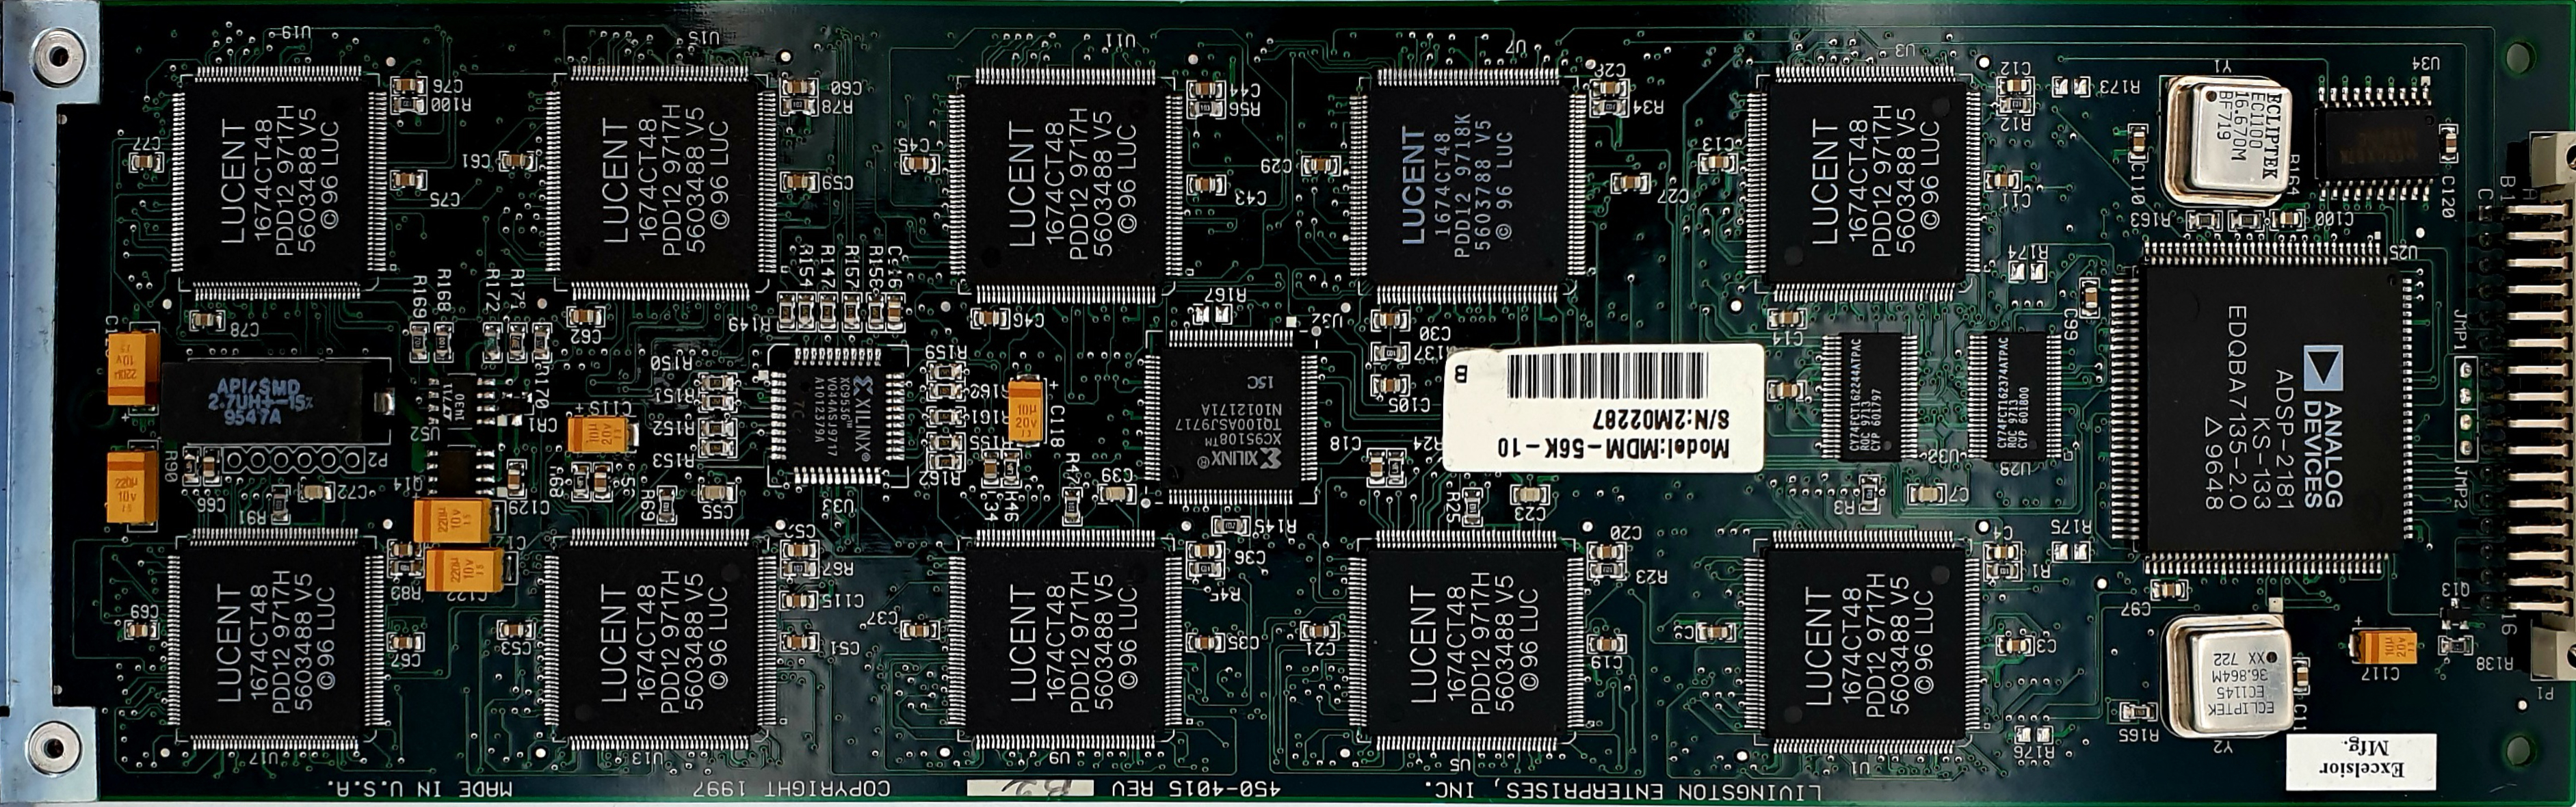
\includegraphics[width=0.9\linewidth]{images/Livingston_Portmaster3_dsp_top.jpg}

\makefooter

\end{document}